
\documentclass[border=3pt]{standalone}

% font set
\usepackage{ctex}
\usepackage{fontspec}
\usepackage[sc]{mathpazo}
\usepackage{anyfontsize}

\setmainfont{SourceSerif4-Regular.ttf}[%
    Path = ../../fonts/,
    BoldFont = SourceSerif4-Bold.ttf,
    ItalicFont = SourceSerif4-It.ttf,
    BoldItalicFont = SourceSerif4-BoldIt.ttf
]
\setCJKmainfont[%
    Path = ../../fonts/,
    BoldFont=SourceHanSansSC-Medium.otf,
    ItalicFont=gkai00mp-2.ttf%
]{SourceHanSansSC-Normal.otf}

% colors
\usepackage[dvipsnames]{xcolor}
\definecolor{pku-red}{RGB}{139,0,18}
\usepackage{colortbl}
\newcommand{\light}[1]{\textcolor{Orchid}{#1}}
\newcommand{\contrastlight}[1]{\textcolor{TealBlue}{#1}}

\usepackage[normalem]{ulem}

\usepackage{makecell}

% math package
\let\Bbbk\relax
\usepackage{amsmath}
\usepackage{mathrsfs}
\usepackage{amssymb}
\usepackage{amsfonts}
\usepackage{stmaryrd}
\usepackage{latexsym}
\usepackage{extarrows}
\SetSymbolFont{stmry}{bold}{U}{stmry}{m}{n}
\allowdisplaybreaks[3]


% math notations
\newcommand{\LHS}{\mathrm{LHS}}
\newcommand{\RHS}{\mathrm{RHS}}
\newcommand{\Z}{\mathbb{Z}}
\newcommand{\N}{\mathbb{N}}
\newcommand{\R}{\mathbb{R}}
\newcommand{\Q}{\mathbb{Q}}
\newcommand{\C}{\mathbb{C}}
\newcommand{\E}{\mathbb{E}}
\renewcommand{\O}{\mathcal{O}}
\newcommand{\id}{\mathrm{id}}
\DeclareMathOperator*{\Span}{Span}
\DeclareMathOperator*{\im}{Im}
\DeclareMathOperator*{\rank}{rank}
\DeclareMathOperator*{\card}{card}
\DeclareMathOperator*{\grad}{grad}
\DeclareMathOperator*{\argmax}{argmax}
\DeclareMathOperator*{\epi}{epi}
\DeclareMathOperator*{\maximize}{maximize}
\DeclareMathOperator*{\minimize}{minimize}
\renewcommand{\d}{\mathrm{d}}
\newcommand{\Pow}{\mathcal{P}}
\newcommand{\cov}{\mathsf{Cov}}
\newcommand{\var}{\mathsf{Var}}
\newcommand{\Nor}{\mathcal{N}}
\newcommand{\U}{\mathcal{U}}
\renewcommand{\t}{\mathsf{T}}
\newcommand{\T}{\top}
\newcommand{\F}{\bot}
\newcommand{\norm}[1]{\left\|#1\right\|}
\newcommand{\inner}[2]{\left\langle{#1},{#2}\right\rangle}
\newcommand{\e}{\mathrm{e}}
\newcommand{\const}{\mathrm{const}}
\newcommand{\scB}{\mathscr{B}}
\newcommand{\scF}{\mathscr{F}}
\newcommand{\G}{\mathscr{G}}
\newcommand{\Exp}{\mathsf{Exp}}
\newcommand{\DExp}{\mathsf{DExp}}
\newcommand{\Lap}{\mathsf{Lap}}
\newcommand{\calP}{\mathcal P}
\newcommand{\calS}{\mathcal S}
\newcommand{\calF}{\mathcal F}
\newcommand{\calM}{\mathcal M}
\newcommand{\KL}{\mathrm{KL}}
\newcommand{\ReLU}{\mathsf{ReLU}}
\newcommand{\val}{\mathsf{val}}

% plots
\usepackage{tikz}
\usetikzlibrary{arrows}
\usetikzlibrary{arrows.meta,positioning,calc,3d}
\usepackage{tikz-3dplot}
\usepackage{pgfplots}
\pgfplotsset{compat=newest}

\begin{document}
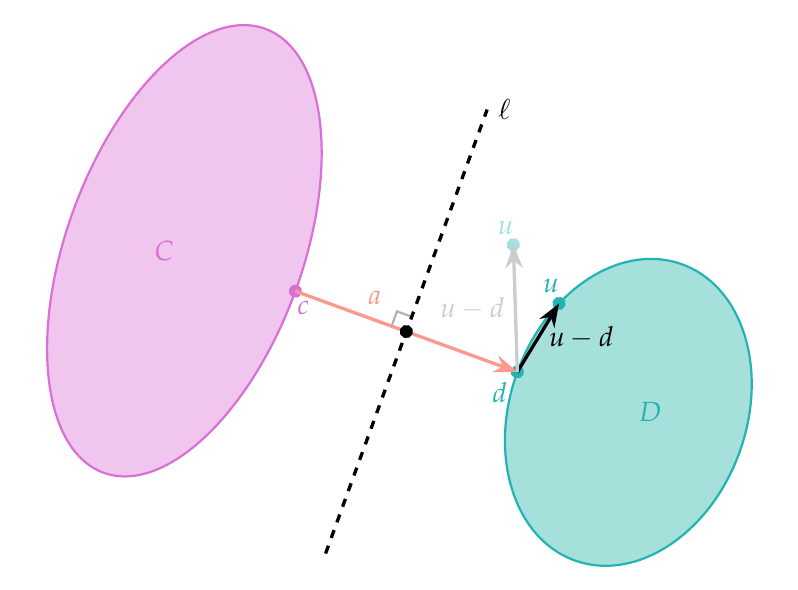
\begin{tikzpicture}[>=Stealth,thick,rotate=-20]

% Draw convex sets C and D
\draw[thick, Orchid,fill=Orchid!40] (-3, 0) ellipse (1.5 and 3) node[left] {$C$};
\draw[thick, TealBlue,fill=TealBlue!40] (3, 0) ellipse (1.5 and 2) node[right] {$D$};

% Points c and d
\filldraw[Orchid] (-1.5, 0) circle (2pt) node[below,xshift=0.1cm] {$c$};
\filldraw[TealBlue] (1.5, 0) circle (2pt) node[below left] {$d$};

\draw[gray!60] (-0.2,0) -- (-0.2,0.2) -- (0,0.2);

% Line connecting c and d
\draw[very thick, ->,Salmon!80] (-1.5, 0) -- (1.5, 0) node[midway, above=0.2cm,xshift=-0.4cm] {$a$};

% Midpoint
\filldraw[black] (0, 0) circle (2pt) node[below] {};

% Perpendicular bisector (Separating Hyperplane)
\draw[dashed,very thick] (0, -3) -- (0, 3) node[right] {$\ell$};

% Additional vectors from c and d
\filldraw[TealBlue] (1.7, 0.9978) circle (2pt) node[above,xshift=-0.1cm] {$u$};
\draw[->, very thick] (1.5, 0) --  node[right] {$u-d$} (1.7, 0.9978);

\filldraw[TealBlue!40] (0.9, 1.5) circle (2pt) node[above,xshift=-0.1cm] {$u$};
\draw[->, very thick,gray!40] (1.5, 0) --  node[left] {$u-d$} (0.9, 1.5);

\end{tikzpicture}
\end{document}
